\section{Multiplayer}
\subsection{Công việc đã làm}
\subsubsection{PvP Off}
Hiện thực PvP Offline có ứng dụng Board Rotator, ứng dụng ISquadProvider để áp đúng Squad cho mỗi người chơi 

\subsubsection{PvP Onl}
\begin{enumerate}
    \item Bước đầu tìm hiểu các phương án Multiplayer.
    \item Thiết lập thành phần tạo phòng
    \item Vận dụng Reliable Data Stream của Photon Fusion, ứng dụng thành phần gửi Move của client.
\end{enumerate}


\subsection{Công việc tương lai}
\begin{enumerate}
    \item Ứng dụng các cơ chế xử lí timeout, disconnect
    \item Thêm chế độ đấu hạng
    \item Thêm các tính năng log-in, link Facebook, Google
\end{enumerate}

\subsection{So sánh giữa hai phương pháp: Fusion Network Object và Fusion Reliable Data}

\begin{center}
\begin{tabular}{ |m{2cm}|m{20em}|m{20em}| } 
    \hline 
    Phương pháp Multiplayer & Fusion Network Object & Fusion Reliable Data \\ \hline
    Phương thức đồng bộ & Đồng bộ từng GameObject ở thời gian thực & Chỉ nhận và gửi dữ liệu ở từng lần gọi hàm \\ \hline
    Băng thông & Lớn, mỗi gói tin cần chứa thêm thông tin Rpc để đến được GameObject đúng & Nhỏ, chỉ chứa đủ thông tin \\ \hline
    Coupling & Đòi hỏi coupling với cấu trúc Model View Controller hiện có & Hoàn toàn decoupled khỏi cấu trúc MVC hiện có, chỉ giao tiếp qua Interface IMoveInputProvider \\ \hline
    Tốc độ & Nhanh, thường được ứng dụng cho các game FPS, RTS & Chậm, thường được ứng dụng cho các game theo lượt \\
    \hline
\end{tabular}
\end{center}

\subsubsection{Kết quả Benchmark}
Sử dụng 10 lần probe để kiểm tra tổng băng thông mỗi phương thức sử dụng:

\begin{center}
\begin{tabular}{ |m{2cm}|m{20em}|m{20em}| } 
    \hline 
    Phương pháp Multiplayer & Fusion Network Object & Fusion Reliable Data \\ \hline
    Tổng băng thông & 320 bytes & 70 bytes \\ \hline
    Average RTT & 194.6 ms & 728.8 ms \\
    \hline
\end{tabular}
\end{center}

\begin{figure}[h!]
    \begin{center}
    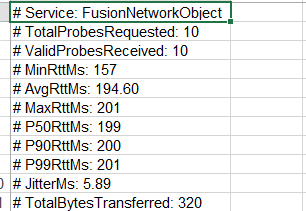
\includegraphics[width=0.5\textwidth]{Content/Multiplayer/networkobjectbench.png}
    \caption{Phương pháp Network Object}
    \end{center}
\end{figure}

\begin{figure}[h!]
    \begin{center}
    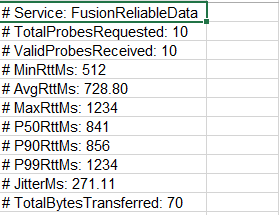
\includegraphics[width=0.5\textwidth]{Content/Multiplayer/reliabledatabench.png}
    \caption{Phương pháp Reliable Data}
    \end{center}
\end{figure}
